\documentclass[tikz,border=5]{standalone}
\usetikzlibrary{positioning}
\tikzset{shape example/.style = {
    color=black!50, draw, fill=blue!10,
    inner xsep=0.5cm, inner ysep=0.5cm,
}}
\begin{document}
\Huge
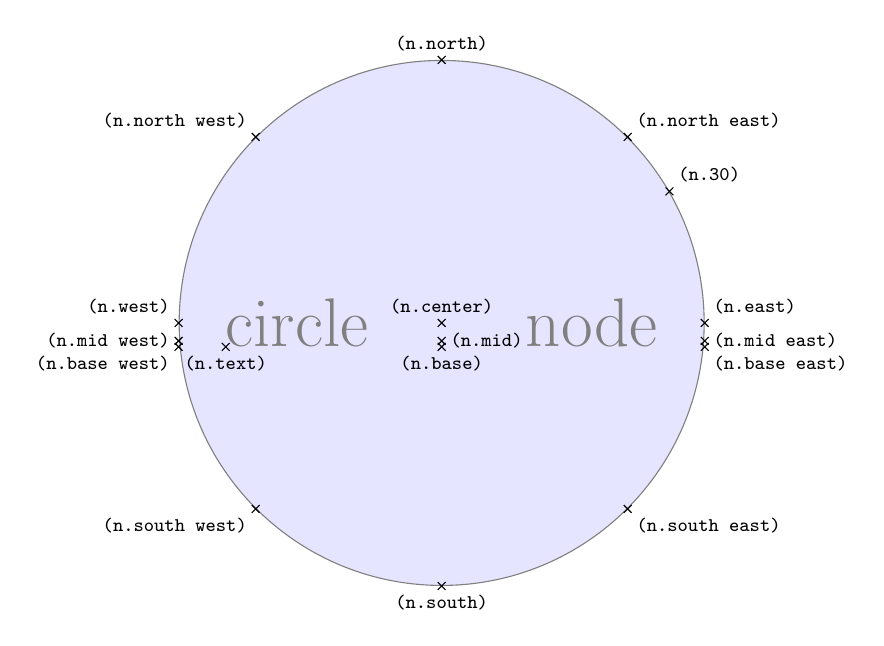
\begin{tikzpicture}[node distance = 1mm]
  \node[name=n,shape=circle,shape example] {\Huge circle\hspace{2cm}node};
  \foreach \anchor/\placement in
    {center/above, text/below, 30/above right,
       mid/right, mid east/right, mid west/left,
       base/below, base east/below right, base west/below left,
       north/above, south/below, east/above right, west/above left,
       north east/above right, south east/below right, south west/below left,
         north west/above left}
      \draw[shift=(n.\anchor)] plot[mark=x] coordinates{(0,0)}
        node[\placement,label distance = 0mm,inner sep=3pt]
          {\scriptsize\texttt{(n.\anchor)}};
\end{tikzpicture}
\end{document}
